\begin{figure}
    \centering
    % 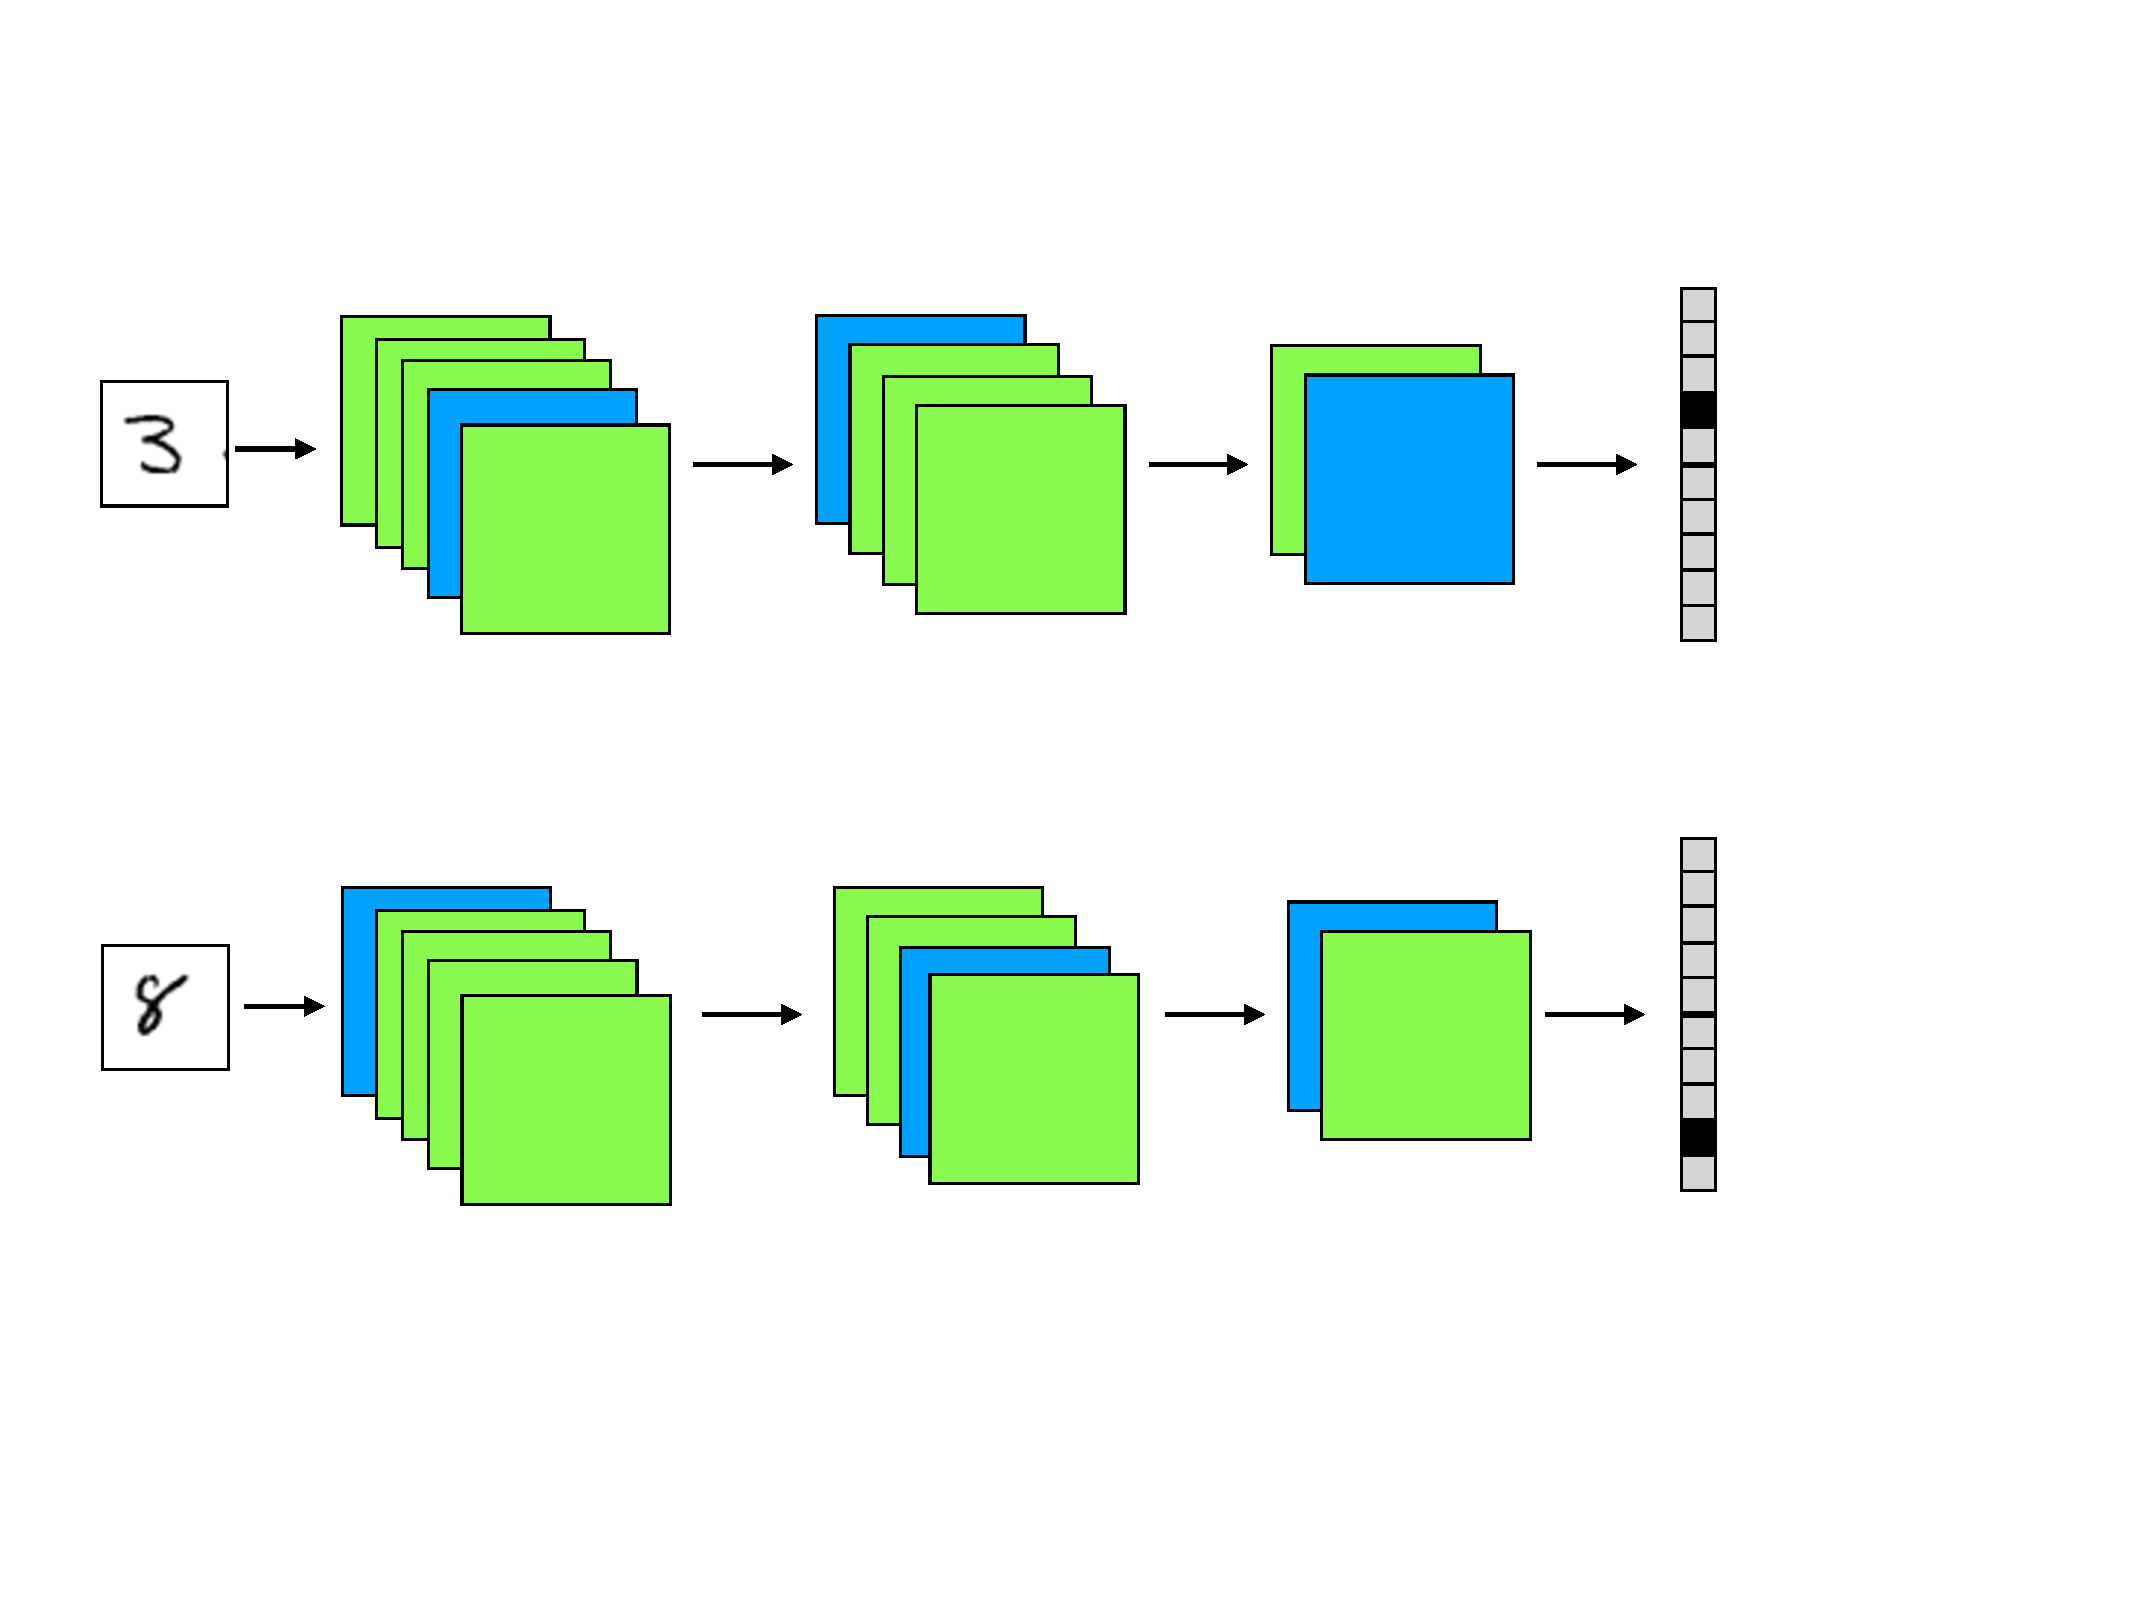
\includegraphics[height=1.5in,trim={1.5cm 5cm 3cm 3.5cm},clip]{figs/layercnn.pdf}
    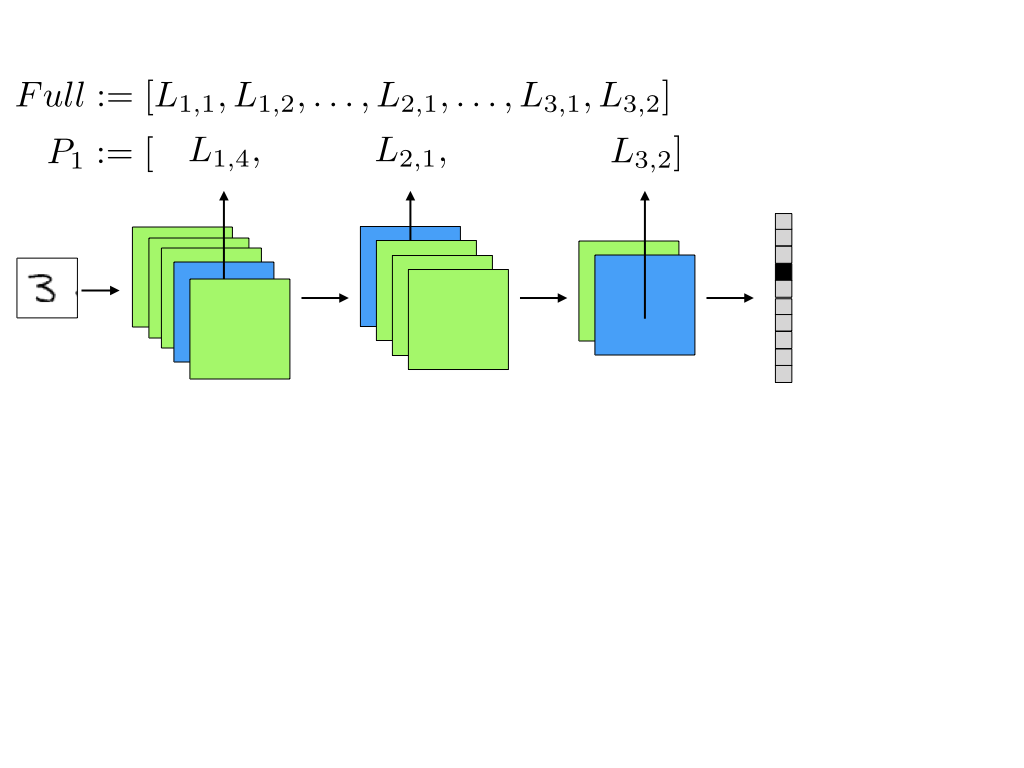
\includegraphics[width=\columnwidth,trim={0cm 12cm 5cm 2.5cm},clip]{5_unlearn/figs/layercnn.png}
    \caption[Conditionally independent network subsets]{\label{fig:main1} Large deep learning networks typically associate specific subsets of network parameters, blocks (blue), to specific samples in the input space.
    Traditional forward or backward passes may not reveal these blocks: high correlations among features may not distinguish important ones. Input perturbations can be used to identify them in a probabilistic, distribution-free manner.}
\end{figure}
\begin{figure}
	\centering
	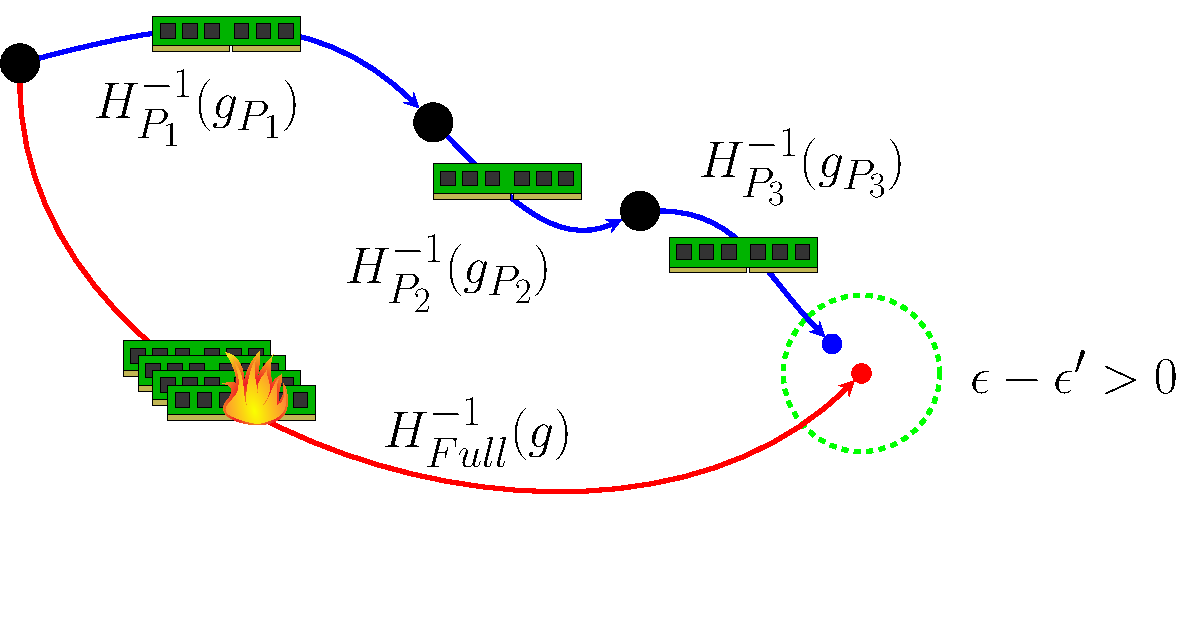
\includegraphics[width=\columnwidth,trim={0cm 1cm 0cm 0cm},clip]{5_unlearn/figs/unlearning_fig.pdf}
	\caption[Efficient unlearning]{\label{fig:main2}Network blocks can be unlearned together in an efficient block-coordinate style update (blue lines), approximating an update to the full network which requires a costly/infeasible full Hessian inverse (red line).}
\end{figure}

\section{Problem Setup for Unlearning}
Let $\cA$ be an algorithm that takes as input a training set $\cS$ and outputs a hypothesis $w \in \cW$, defined by a set of $d$ parameters $\Theta$. 
An unlearning scheme $\cU$ takes as input a sample $z' \in \cS$ used as input to $\cA$, and ideally, outputs an \textbf{updated} hypothesis $w' \in \cW$ where $z'$ has been deleted from the model.
%
% Clearly within unlearning we do not wish to simply rerun $\cA$ on the subset without the sample to delete.
% Particularly for modern machine learning problems with extremely large datasets and model architectures, retraining can be costly or impossible.
%
% Retraining may be costly or impossible, but provides a baseline oracle to which we can compare updates as in \eqref{eq:unlearn}.
% However, this provides a baseline with which we can compare any other potential unlearning algorithm to.
% Namely, a
An unlearning algorithm should output a hypothesis that is close or equivalent to one that would have been learned had the input to $\cA$ been $\cS \setminus z^\prime$. A framework for this goal was given by \cite{ginart2019making} as,
% Following \cite{sekhari2021remember}, 
\begin{definition}[$(\epsilon,\delta)-$ forgetting]\label{def:forget}
For all sets $\cS$ of size $n$, with a ``delete request'' $z' \in \cS$, an unlearning algorithm $\cU$ is $(\epsilon, \delta)-$forgetting if
\begin{align}
\PP(\cU(\cA(S), z') \in \cW) \leq e^\epsilon\PP(\cA(\cS\setminus z') \in \cW) + \delta
\end{align}
\end{definition}
In essence, for an existing model $w$, a good unlearning algorithm for request $z' \in \cS$ will output a model $\hat{w}$ close to the output of $\cA(S \setminus z')$ (retraining without that sample) with high probability.

\begin{remark}
Definition \ref{def:forget} is similar to the standard definitions of differential privacy. The connection to unlearning is: if an algorithm is $(\epsilon, \delta)-$forgetting for unlearning, then it is also differentially private. 
\end{remark}

%\cite{unlearning} provide a straightforward algorithm for mild assumptions under the structure of the algorithm $\cA$.
If $\cA$ is an empirical risk minimizer for the loss $f$, let
\begin{align}
    \cA : (\cS, f) \rightarrow \hat{w},% \nabla^2 F(\hat{w}),
\end{align}
$\hat{w} = \arg\min F(w)$ and $F(w) = \frac{1}{n}\sum_{i=1}^n f(w, z_i).$ 
%$\nabla^2 F(\hat{w})$ is the Hessian of the empirical loss at the minimizer $\hat{w}$.
% Ideally, we would like to perform a ``one-shot" update to $\hat{w}$, in the same way we may update model parameters in a traditional forward learning setting. Consider the following \textit{one-shot unlearning update}:
% \begin{align}\label{eq:bbunlearn}
    % \tilde{w} = \hat{w} + g(z^\prime).
% \end{align}
Recall $g(z')$ from \eqref{eq:unlearn}:  
our unlearning task 
essentially involves 
identifying 
the form of $g(z')$ for which the update in \eqref{eq:unlearn} is $(\epsilon,\delta)$-forgetting. If an oracle provides this information, we have 
accomplished the unlearning task.

The difficulty, 
as expected, tends to 
depend on $f$ and $\cA$. 
Recent unlearning results have identified forms of $f$ and $\cA$ where such a $g(z')$ exists. The authors in \cite{sekhari2021remember} define $g(z') = \frac{1}{n-1}H'^{-1}\nabla f(\hat{w},z')$, where
%Given this, they provide an unlearning algorithm $\cU$ with the update for each $z \in T$:
\begin{align}\label{eq:sekhariunlearn}
    H' &= \frac{1}{n-1} \left(n\nabla^2 F(\hat{w}) - \nabla^2 f(\hat{w},z')\right),
%    \bar{w} &= \hat{w} + \frac{1}{n-1} (\hat{H})^{-1} \nabla f(\hat{w},z) \\
%    \tilde{w} &= \hat{w} + N(0,\sigma^2 I)
\end{align}
with additive Gaussian noise $w' = w' + N(0,\sigma^2)$ scaling as a function of $n, \epsilon, \delta$, and the Lipschitz and (strong) convexity parameters of the loss $f$. We can interpret the update using \eqref{eq:sekhariunlearn} from the optimization perspective as a trajectory ``reversal'': starting at a random initialization, the first order (stochastic gradient) trajectory of  ${w}$ {\em with}  $z'$ is reversed using {\em residual} second order curvature (Hessian) information at the optimal $\hat{w}$ in \eqref{eq:sekhariunlearn}, achieving unlearning. This is shown to satisfy Definition~\ref{def:forget}, and only incurs an additive error that scales by $O(\sqrt{d}/n^2)$ in the gap between $F(w')$ and the global minimizer $F(w^*)$ over the ERM $F(\hat{w})$. 

\paragraph{Rationale for approximate schemes.}
% From the optimization reversal perspective, it is clear that there may be other choices to achieve unlearning.
The aforementioned update requires storing, computing, and inverting the $O(d^2)$ Hessian matrix.
For a practitioner interested in unlearning, this can only be directly instantiated if one has extensive computational resources.
In settings where it is not directly possible to compute the Hessian inverse necessary for $H'^{-1} \nabla f(\hat{w},z')$, we must consider alternatives. 

\paragraph{A potential idea.} Our goal is to identify a form of $g(z')$ that \textbf{approximates} the Hessian-scaled gradient $H'^{-1} \nabla f(\hat{w},z')$. 
Let us consider the Newton-style update suggested by 
\eqref{eq:sekhariunlearn}
as a smoothing of a traditional first order gradient step. 
The inverse Hessian is a weighting matrix,
appropriately scaling the gradients based on the second order difference between the training set mean point $F(\hat{w})$ and the sample of interest $f(\hat{w},z')$. 
This smoothing can also be viewed from an information perspective:
the Hessian in this case corresponds to a Fisher-style information matrix, and its inverse as a conditional covariance matrix \citep{Golatkar_2021_CVPR,golatkar2020forgetting}.
It could be possible that, if there are a \textbf{specific set of parameters} that have {\em small gradients} at $f(\hat{w},z')$, or if the information matrix is zero or small, then we need not consider their effect. 

\paragraph{Examples of this intuition in vision.} \cite{bau2017network,fong2018net2vec,Sun_2019_ICCV} and others have shown that models trained on complex tasks tend to \textit{delegate} subnetworks to specific regions of the input space. That is, parameters and functions within networks tend to (or can be encouraged to) act in \textit{blocks.}
For example, activation maps for different filters in a trained (converged) CNN model show differences for different classes, especially for filters closer to the output layer.
We formalize this observation as an assumption for samples in the training set.

\begin{assumption}\label{assum:sub}
For all subsets of training samples $S \subset \cS$, there exists a subset of trained model parameters $P^* \subset \Theta$ such that
\begin{align}\label{eq:assum}
    f(S)\ \bot w_{\Theta\setminus P}^*\ |\ w_{P}^*
\end{align}
\end{assumption}
Due to the computational issues discussed above, 
if we could make such a simple/principled selection scheme practical, it may offer significant 
benefits.


%Consider the following generalization of the second line of \ref{eq:unlearn}:
%\begin{align}\label{eq:bbunlearn}
%    \bar{w} = \hat{w} + G^\prime\nabla f(\hat{w},z),
%\end{align}
%where $G$ is a some scaling matrix meant to represent the necessary scaling necessary to unlearn the sample $z$ from parameters as appropriate.


%While practical for problems of reasonable dimension, clearly this algorithm is heavily dependent on storing, computing, and inverting the $O(d^2)$ Hessian matrix. For deep learning settings where the dimension of the problem scales to millions of parameters, this algorithm is infeasible. Furthermore, inversion of the updated Hessian at scale will lead to large amounts of instability if even mild assumptions regarding the loss do not hold, or the amount of noise necessary to satisfy these assumptions will completely destroy any predictive power the the model originally had.